\chapter{Introduction}
%\pagestyle{chapter}
\begin{shadequote}
The sure and definite determination (of species of bacteria) requires so much time, so much acumen of eye and judgement, so much of perseverance and patience that there is hardly anything else so \mbox{difficult}. \par--\emph{Otto F. M\"uller}
\end{shadequote}


\section{Description of Problem}
The quote above, by no mistake, graced the cover of the International Journal of Systematic and Evolutionary Microbiology for decades.
Whereas plant and animal systematists are guided by a theory based approach to \index{demarcating} species, microbiologists have yet to agree on a set of ecological and evolutionary properties that could serve to identify bacterial species~\cite{cohan2007systematics}.
They are naturally handicapped by the paucity of morphological differences that could aide in differentiation of closely related bacterial species.
Another factor is that microbiologists cannot predict which traits will cause a speciation event since bacteria are capable of receiving genes from distant relatives through a process known as horizontal gene transfer (HGT)~\cite{cohan2007systematics}.
Thus, in order to effectively understand the microbiome we must strive towards developing a method for consistently demarcating groups, from bacterial diversity, that play distinct ecological roles~\cite{koeppel2008identifying}.

Initially, closely related bacterial species were identified based on metabolic phenotype.
Systematists now rely on molecular approaches that utilize the decreasing cost of DNA sequencing to compare genetic information.
A 70\% cutoff was established for whole genome hybridization studies (comparing loss and gain of large chunks of DNA), replaced by varying degrees of sequence identities in homologous genes~\cite{cohan2007systematics,carlo,staley1997biodiversity}.
From these technological breakthroughs scientists have taken great steps towards understanding bacteria speciation, at the same time they have brought into focus new difficulties.

\subsection{Diversity of Bacterial Species}
Modern molecular techniques have revealed an extraordinary diversity of microorganisms, most of which are as yet uncharacterized~\cite{bohannan2003new}.
Estimates of eukaryotic diversity fall within the range of 10 to 50 million species. Even though we have only observed approximately 9000 prokaryotic species, indirect approaches that do not rely on cultivation hint at the existence of a billion or more prokaryotic species worldwide and 10 million within a given habitat~\cite{cohan2008origins}.
To observe biodiversity through molecular means, scientists should find organisms in highly distinct sequence clusters, since each cluster has had a long history of separate evolution they have likely evolved unique adaptations shared by the entire cluster~\cite{cohan2007systematics}.
The only rational approach to clustering such a large group of diverse organisms effectively is with a theory based molecular method.

Current protocols for deciding bacterial lineage are functionally incomplete. Recent ecological studies show that a named bacterial species is typically an assemblage of closely related but ecologically distinct populations~\cite{cohan2007systematics}.
Thus, within a named species established by antiquated methods, one may find distantly related organisms that do not naturally fit in with what we define to be a cohesive species cluster, which contradicts ideal approaches to biodiversity discovery.
Comprehensive study is impossible.

Fortunately, however, organisms from every known community appear to cluster into discrete ecologically interchangeable individuals~\cite{cohan2007systematics}.
Our envisioned demarcation algorithm would be capable of identifying putative clusters of ecologically distinct organisms within named bacterial clades.
While accuracy is of utmost importance, due to the large numbers of potential bacterial species we would appreciate an efficient demarcation algorithm.

\begin{figure}
\centering
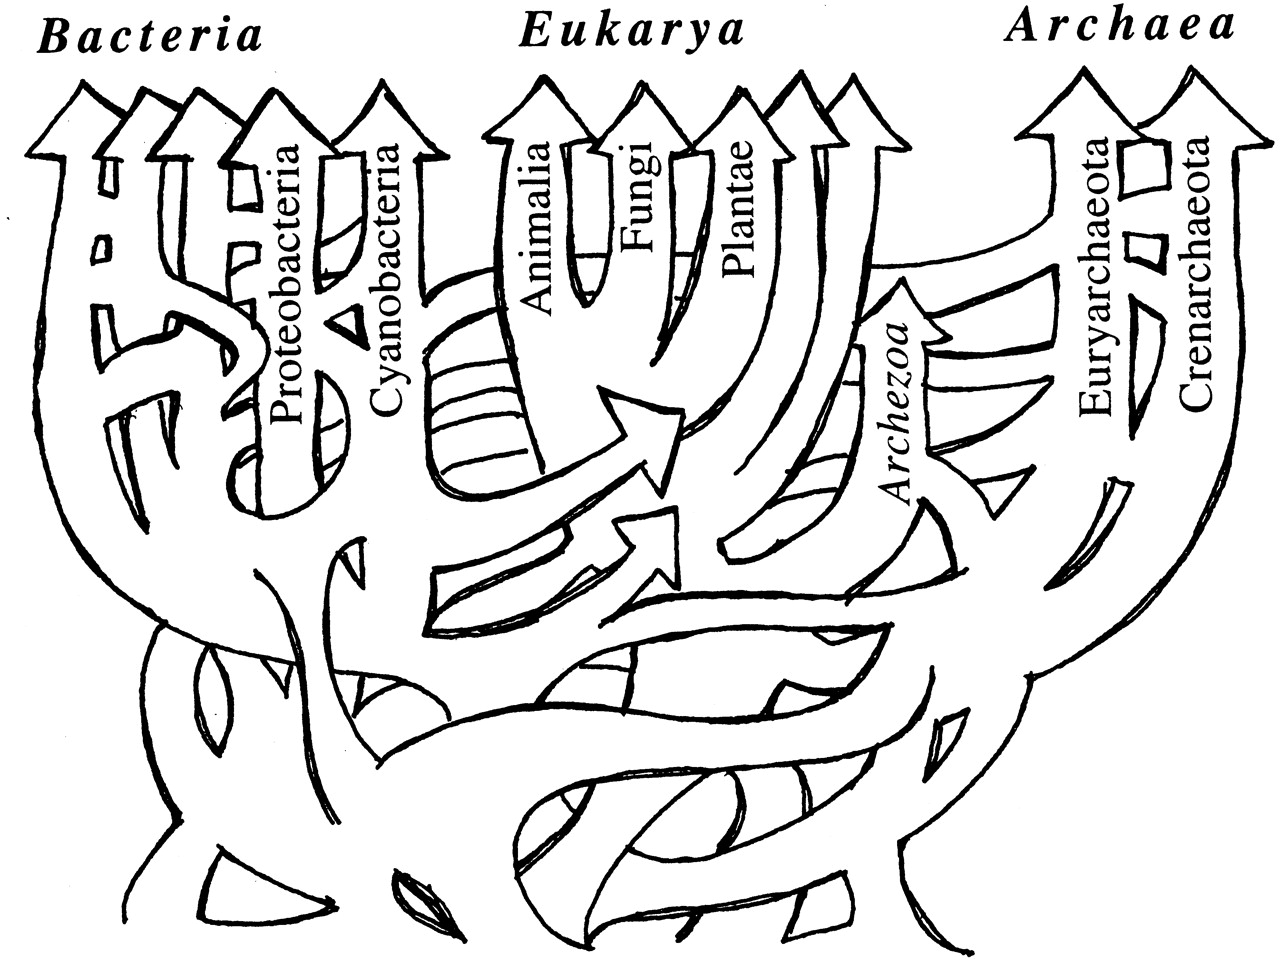
\includegraphics[scale=0.25]{images/HGTTree-CH1}
\label{fig:HGTmodel}
\caption[Possible model tree representing HGT]{Possible model tree representing HGT (reprinted from\protect\cite{doolittle1999phylogenetic}).}
\label{fig:HGTmodel}
\end{figure}

\subsection{Differences of Bacterial Population Dynamics}
As briefly mentioned earlier there exist peculiarities of bacterial population dynamics that complicate demarcation.

\subsubsection*{Asexual reproduction}
Prokaryotes have the ability to reproduce clonally.
In fact, genetic exchange occurs typically through processes not tied to reproduction.
Thus, sexual isolation is not a pre-requisite for permanent divergence between distinct ecological bacterial populations ~\cite{cohan2007systematics}.
This means that sympatric speciation becomes a common occurrence.
Early models for understanding adaptation, evolution, and speciation in these organisms often focused on clonality and periodic selection~\cite{gogarten2002prokaryotic}.
Genetic exchange plays a different role in evolution from that in plants and animals, because it is estimated to be very rare, and only small amounts.
Also, mutations in haploid bacteria will immediately be phenotypically expressed, resulting in rapid displacement of a parental genotype~\cite{staley1997biodiversity}.

\subsubsection*{Horizontal Gene Transfer (HGT)}
In contrast to eucaryotes, bacterial genetic features can be transferred among quite distantly related bacteria via various genetic exchange mechanisms such as transformation and conjugation.
Genetic features may reside in the cell on a plasmid or become incorporated into the bacterial chromosome~\cite{staley1997biodiversity}.
HGT can occur between even very distantly related organisms, e.g., between bacteria and plants or fungi~\cite{gogarten2002prokaryotic} (see Figure~\ref{fig:HGTmodel}).
It leads to genomes whose constituent genes have different evolutionary histories~\cite{gogarten2002prokaryotic}.

\section{Practical Applications}
We must first be able to identify the basic units operating within the system, in order to understand the microbiome.
Once we have established the atomic functional unit we can then start building collections of relationships between these units. 

\subsubsection*{Antibiotic resistance and other health benefits}
Preparing for future epidemics, we should try and discover all long-standing ecotype diversity within each named pathogenic species, allowing us to anticipate disease-causing properties of each ecotype~\cite{cohan2007systematics}.
Partially due to poor antibiotic management, we may be entering an age similar to when antibiotics were not available.

\subsubsection*{Biotechnology}
After discovering a strain with a valuable enzyme, one could then search for homologs in each ecotype closely related to the strain, potentially allowing discovery of similar enzymes with different substrates or with optima at different conditions~\cite{cohan2007systematics}.
This is particularly a useful concept for developing improved biofuel producing bacteria.
Microbial fuel cells hold great promise as a sustainable biotechnological solution to future energy needs, however current efforts to improve the efficiency of such fuel cells are limited by the lack of knowledge about the microbial ecology of these ecosystems~\cite{rabaey2004biofuel}

Improved biocatalysts and cellulase preparations are the major technical roadblocks to building a successful bioethanol industry~\cite{dien2003bacteria}.

\subsubsection*{True quantification of ecological diversity within a community}
Microbial ecologists are often interested in the factors that regulate community diversity across temporal and spatial scales, the impact of human activity on this diversity and the consequences of this diversity for ecosystem processes~\cite{bohannan2003new}.
An Ecotype-Based Systematics has been proposed for identifying ecotypes, the fundamental units of bacterial ecology and evolution.
Scientists suggest that by creating a third name describing a species discovered ecotype the fullness of ecological diversity within the bacterial world will be taken most seriously~\cite{cohan2007systematics}.
They also predict that identifying taxa at the level of ecotypes, systematics will allow microbiologists to optimize their choice of sequencing targets.
From a sample one can determine how representative it is of the environment~\cite{bohannan2003new}.
Ideally, one should choose organisms from different ecotypes to get a fuller gene content survey of the ecosystem~\cite{cohan2007systematics}.
As mentioned, current methods for surveying diversity involve binning and assigning a an operational taxonomic unit without a theoretical justification.
Ecotype demarcation will allow quantification of the ecological diversity within a community; a step toward understanding the plethora of ecological interactions within natural microbial communities~\cite{cohan2007systematics}.

\subsubsection*{Simplify the burden of industrial testing of bacterial strains for their safety and efficacy in agricultural applications}
For example, for any named species that is heterogeneous for characteristics of safety concern (such as secreted metabolites and persistence in the environment) the European Union requires that any new strain developed for release be tested for these characteristics of concern.
However, individual strains from a species known to be homogeneous for these features need not be tested, thus demarcating taxa as ecologically homogeneous units would obviate or at least lessen the burden of these tests~\cite{cohan2007systematics}.

\subsubsection*{Bioremediation}
Bioremediation has the potential to restore contaminated environments inexpensively yet effectively, but a lack of information about the factors controlling growth and metabolism of microorganisms in polluted environments often limits its implementation~\cite{lovley2003cleaning}.
Combining models that can predict the activity of microorganisms that are involved in bioremediation with existing geochemical and hydrological models should transform bioremediation from a largely empirical practice into a science~\cite{lovley2003cleaning}.

\section{Demarcation Software}
Today there are several freely available demarcation programs available: Ecotype Simulation (ES1), BAPS, GMYC, AdaptML, and newly introduced Ecotype Simulation 2 (ES2) , which is an improvement on ES1.
Each is an attempt to define species as a fundamental unit, usable in practical applications just mentioned.
They all differ in background theory, resulting in different demarcations.
I will focus specifically on ES1 and the improvements resulting in ES2, then explore a few of the differences between programs that result in each demarcation solution.


\section{Outline}
My aims for this project are several.
The final result should be a production ready version of the optimized Ecotypes Simulation (ES2) software.
However, first we plan on carrying out several tests to show ES2 is accurate, and efficient.
I will run ES2 through the same previous test parameters the Cohan lab used to test ES1 to compare all demarcation algorithms on small inputs.
This includes generated datasets and environment collected sequences.
It is important to demonstrate similar accuracy scores of ES2 to ES1.
We hypothesized that the new, more efficient, demarcating algorithm within ES2 will not significantly affect the accuracy of our output.
Next, I want to identify the new reasonable upper limit for input size (i.e., number of sequences) for ES2.
Then I will run ES2 in conjunction with other available demarcation programs (BAPS, GMYC, AdaptML) on large generated datasets (up to the newly established reasonable limit) and evaluate demarcation algorithm accuracy and speed.

Chapter 1 introduced the problem that ES tries to address, and the benefits that understanding bacterial speciation will achieve.
The following chapter will go over several current molecular models for bacteria speciation, the underlying algorithms that make them function, and describe the design of ES.
Next section discusses our approach to ES optimization, as well as other future enhancements planned.
In the fourth chapter, I will go over comparison results between various demarcation programs.
Finally, the conclusion will contain a discussion of what we set out to accomplish compared to what we achieved, shortcomings, and some final thoughts on future directions.

